%% LyX 2.1.4 created this file.  For more info, see http://www.lyx.org/.
%% Do not edit unless you really know what you are doing.
\documentclass[a4paper,twoside,czech,czech,cleardoublepage=empty,BCOR15mm,DIV12]{scrreprt}
\usepackage{tgtermes}
\usepackage{tgheros}
\usepackage{tgcursor}
\usepackage{newtxmath}
\usepackage[T1]{fontenc}
\usepackage[utf8]{inputenc}
\usepackage{babel}
\usepackage{float}
\usepackage{url}
\usepackage{graphicx}
\usepackage[unicode=true,pdfusetitle,
 bookmarks=true,bookmarksnumbered=false,bookmarksopen=false,
 breaklinks=false,pdfborder={0 0 1},backref=false,colorlinks=false]
 {hyperref}

\makeatletter

%%%%%%%%%%%%%%%%%%%%%%%%%%%%%% LyX specific LaTeX commands.
\pdfpageheight\paperheight
\pdfpagewidth\paperwidth

\newcommand{\noun}[1]{\textsc{#1}}
\floatstyle{ruled}
\newfloat{algorithm}{tbp}{loa}[chapter]
\providecommand{\algorithmname}{Algoritmus}
\floatname{algorithm}{\protect\algorithmname}

%%%%%%%%%%%%%%%%%%%%%%%%%%%%%% User specified LaTeX commands.
%<-------------------------------společná nastavení------------------------------>
\usepackage[numbers,sort&compress]{natbib} %balíček pro citace literatury  
\usepackage{algorithmic}
\usepackage{color}%kvůli barvám ČVUT
\newcommand{\BibTeX}{{\sc Bib}\TeX}%BibTeX logo
\usepackage{multicol}




%<-----------------------------volání stylů----------------------------------------->
% (znak % je označení komentáře: co je za ním, není aktivní)

%<--------matematické písmo--------------------------------------->

%\usepackage[helvet]{packages/sfmath}%matematika ala helvetica



%<------------------------------záhlaví stránek------------------------------------>
%\usepackage{packages/bc-headings}
\usepackage{packages/bc-fancyhdr}

%<------------------------------hlavičky kapitol------------------------------------>
%\usepackage{packages/bc-neueskapitel}
\usepackage{packages/bc-fancychap}

\makeatother

\begin{document}
~\thispagestyle{empty}\begin{center}\pagenumbering{roman}\vspace{10mm}


\textsf{\textsc{\noun{\LARGE{}České vysoké učení technické v Praze}}}\\
\vspace{0.5em}
\textsf{\textsc{\noun{\LARGE{}Fakulta elektrotechnická}}}\\
\vspace*{1em}
\textsf{\textsc{\noun{\Large{}katedra kybernetiky}}}\vspace{15mm}


%%% Aby vložení loga  správně fungovalo, je třeba mít soubor lev.png nahraný v pracovním adresáři,
%%% tj. v adresáři, kde se nachází překládaný zdrojový soubor. 

\includegraphics[width=0.3\textwidth]{obrazky/lev}\vspace{15mm}


\textsf{\huge{}BAKALÁŘSKÁ/DIPLOMOVÁ PRÁCE}{\huge \par}

\vspace{15mm}


\textsf{\LARGE{}Název práce}{\LARGE \par}

\vspace{10mm}


\end{center} 

\vspace*{\fill}


\vspace{10mm}

\begin{description}
\item [{{\large{}Autor:}}] \noindent \textsf{\large{}Matěj Račinský}{\large \par}
\item [{{\large{}Vedoucí~práce:}}] \noindent \textsf{\large{}Dr. Martin
Saska}{\large{}\hfill{}}\textsf{\large{}Praha,}{\large{} \the\year % nebo doplňte rok vzniku vaší bakalářské práce
}{\large \par}
\end{description}
\clearpage{}

{\small{}\thispagestyle{plain}\addcontentsline{toc}{chapter}{Abstrakt} }{\small \par}

\noindent {\small{}~\vfill{}
}{\small \par}
\begin{description}
\item [{{\small{}Název~práce:}}] \noindent {\small{}Název bakalářské práce}{\small \par}
\item [{{\small{}Autor:}}] \noindent {\small{}Matěj Račinský}{\small \par}
\item [{{\small{}Katedra~(ústav):}}] \noindent Kate{\small{}dra kybernetiky}{\small \par}
\item [{{\small{}Vedoucí~bakalářské~práce:}}] \noindent Dr. Martin Saska
\item [{{\small{}e-mail~vedoucího:}}] \noindent {\small{}saska@labe.felk.cvut.cz}\\
{\small \par}
\item [{{\small{}Abstrakt}}] \noindent {\small{}V předložené práci studujeme...
Uvede se abstrakt v rozsahu 80 až 200 slov. Lorem ipsum dolor sit
amet, consectetuer adipiscing elit. Ut sit amet sem. Mauris nec turpis
ac sem mollis pretium. Suspendisse neque massa, suscipit id, dictum
in, porta at, quam. Nunc suscipit, pede vel elementum pretium, nisl
urna sodales velit, sit amet auctor elit quam id tellus. Nullam sollicitudin.}{\small \par}
\item [{{\small{}Klíčová~slova:}}] \noindent {\small{}klíčová slova (3
až 5)}\\
{\small \par}
\item [{\rule[0.5ex]{1\linewidth}{1pt}}]~{\small \par}
\item [{{\small{}Title:}}] \noindent {\small{}Název bakalářské práce v
angličtině}{\small \par}
\item [{{\small{}Author:}}] \noindent {\small{}Matěj Račinský}{\small \par}
\item [{{\small{}Department:}}] \noindent {\small{}Department of Cybernetics}{\small \par}
\item [{{\small{}Supervisor:}}] \noindent Dr. Martin Saska
\item [{{\small{}Supervisor's~e-mail~address:}}] \noindent {\small{}saska@labe.felk.cvut.cz}\\
{\small \par}
\item [{{\small{}Abstract}}] \noindent {\small{}In the present work we
study ... Uvede se anglický abstrakt v rozsahu 80 až 200 slov. Lorem
ipsum dolor sit amet, consectetuer adipiscing elit. Ut sit amet sem.
Mauris nec turpis ac sem mollis pretium. Suspendisse neque massa,
suscipit id, dictum in, porta at, quam. Nunc suscipit, pede vel elementum
pretium, nisl urna sodales velit, sit amet auctor elit quam id tellus.
Nullam sollicitudin. Donec hendrerit. Aliquam ac nibh. Vivamus mi.
Sed felis. Proin pretium elit in neque. Pellentesque at turpis. Maecenas
convallis. Vestibulum id lectus. }{\small \par}
\item [{{\small{}Keywords:}}] \noindent {\small{}klíčová slova (3 až 5)
v angličtině}{\small \par}
\end{description}
\cleardoublepage{}\thispagestyle{empty}~{\small{}\addcontentsline{toc}{chapter}{Zadání
práce} }{\small \par}

\thispagestyle{plain}

{\small{}%\setcounter{page}{3} % nastavení číslování stránek
\ }{\small \par}

\noindent {\small{}\vfill{}
 % nastavuje dynamické umístění následujícího textu do spodní části stránky
~}{\small \par}

\noindent {\small{}Prohlašuji, že jsem svou bakalářskou práci napsal(a)
samostatně a výhradně s použitím citovaných pramenů. Souhlasím se
zapůjčováním práce a jejím zveřejňováním.}{\small \par}

{\small{}\bigskip{}
}\noindent {\small{} V Praze dne \today\hspace{\fill}Jméno Příjmení
+ podpis}\\
{\small{} % doplňte patřičné datum, jméno a příjmení
}{\small \par}

{\small{}%%%   Výtisk pak na tomto míste nezapomeňte PODEPSAT!
%%%                                         *********
}{\small \par}

{\small{}\tableofcontents{}% vkládá automaticky generovaný obsah dokumentu
}{\small \par}


\chapter[Algorithm]{Algorithm}

Basis of whole algorithm is here in pseudocode

\begin{algorithm}
\caption{Basis of whole algorithm}


\begin{algorithmic}[1]

\STATE map := configuration.getMap();

\STATE map := amplifyObstacles(map);

\STATE nodes := mapToNodes(map);

\STATE paths := createGuidingPaths(nodes);

\STATE rrtPath := rrtPath(paths, map, nodes);

\STATE lastState := getBestFitness(rrtPath, map);

\STATE path := getPath(lastState);

\STATE path = straightenCrossingTrajectories(path);

\STATE path := optimizePathByDubins(rrtPath, map);

\end{algorithmic}
\end{algorithm}


Configuration variable is instance of Configuration class, which holds
all configuration variables, including selected map. Map holds all
Aeras of Interest (AoI) and obstacles. All obstacles and AoIs are
represented now as rectangles.

Even if we want to find as short path to AoI as possible, path too
near to obstacles is not convenient for realization, because UAVs
do not use car like motion model used in this simulation, so they
can not exactly follow found trajectories. So in real environment,
it is convenient for the swarm to have path planned with safe distance
from obstacles. Because of that fact, we need to increase size od
obstacles, which is done in line 2 in function amplifyObstacles. 

Line 3 represents discretization of map to graph. Discretizaion divides
map to squares with size set in configuration and eac square is represented
by node. In this graph, there are 4 types of nodes: Free, Obstacle,
UAV and Goal. If part of square of whole square is covered by obstacle,
corresponding node has type Obstacle. If part of square or whole square
is covered by AoI, corresponding node has type Goal. If square contains
UAV, corresponding node has type UAV and rest of squares have corresponding
nodes qith type Free. 

Edges in this graph are only between nodes of neighboring squares,
so each node has maximally 8 edges. Obstacle nodes do not have any
edges.

After converting map to nodes, optional grouping of goals for guiding
path can be turned on. I will cover the grouping in chapter \ref{chap:Modifications-of-goal}.

Line 4 calculates the guiding paths for rrt path algorithm using the
A{*} algorithm. Algorithm has modified cost function and in addition
to cost function of A{*} algorithm, cost of current node is added
during the calculation. Nodes neighboring with obstacles has bigger
cost than nodes which do not have obstacles as neighbors. Thanks to
this modification, guiding path avoids obstacles and has bigger distance
to obstacles. 

On line 5 the rrt path algoritm takes place. This function returns
structure with tree with root at starting position of UAVs and with
array containing leaves of this three, where all UAVs are in Areas
of Interest. 

On line 6 the leaf, where UAVs have best coverage of AoI is chosen.
Quality of coverage is determined by cost function, which will be
mentioned later.\marginpar{todo: možná sem odkaz na kapitolu}

On line 7 the path is built from last state.

On line 8 is optional preparation before optimization using Dubins
maneuvers. In the preperation, all crossings of paths of individual
UAVs are straigtened, so UAVs do not cross other UAVs trajectories
during whole path. During implementation of this method were complications,
which are covered in chapter, and thus the row was removed from the
algorithm. \ref{chap:Paths-narrowing}

On line 9 is optimization by Dubins maneuvers. Optimizations is covered
in chapter.\marginpar{todo: možná sem odkaz na kapitolu}


\chapter[Grouping of goals for guiding path]{Grouping of goals for guiding path\label{chap:Modifications-of-goal}}

During this processing of map (method MapProcessor::getEndNodes in
codebase) all AoIs are grouped to one big AoI, which is the smallest
rectangle covering all AoIs. 

If this modification is turned on, instead of one goal for every AoI
(node in middle of AoI rectangle is considered as goal node), only
one goal is used for all AoIs. This prevents swarm to split and whole
swarm has only one guiding path. The main reason to have one big swarm
instead of more smaller swarms is that smaller swarms (or individual
UAVs in case of same count of AoI and UAVs) is relative localization,
which can be used better when having only one swarm.

Below are images of maps with goals and obstacles. Goals have grren
color and obstacles have grey color.

This approach has advantage, when individual AoIs are near the global
goal of big AoI, as seen in \ref{fig:Maps-with-goals}. 

Disadvantage of this method is, when individual AoIs have big distance
from each other than can be covered by UAVs, this approach totally
fails, because RRT-Path, which is much faster than RRT, has goal very
distant from AoIs, as can be seen in \ref{fig:Map-with-goals}.

\begin{figure}
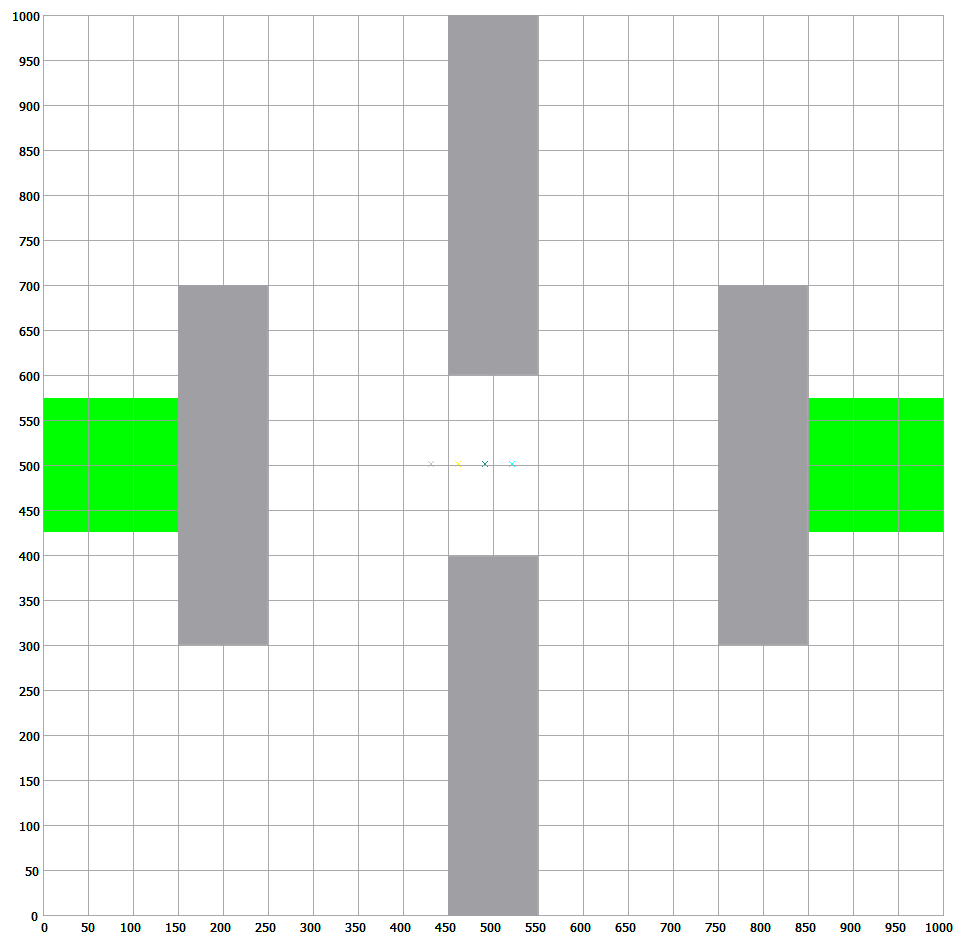
\includegraphics[scale=0.3]{obrazky/map1}

\caption{Map with goals unsuitable for grouping \label{fig:Map-with-goals}}
\end{figure}


\begin{figure}
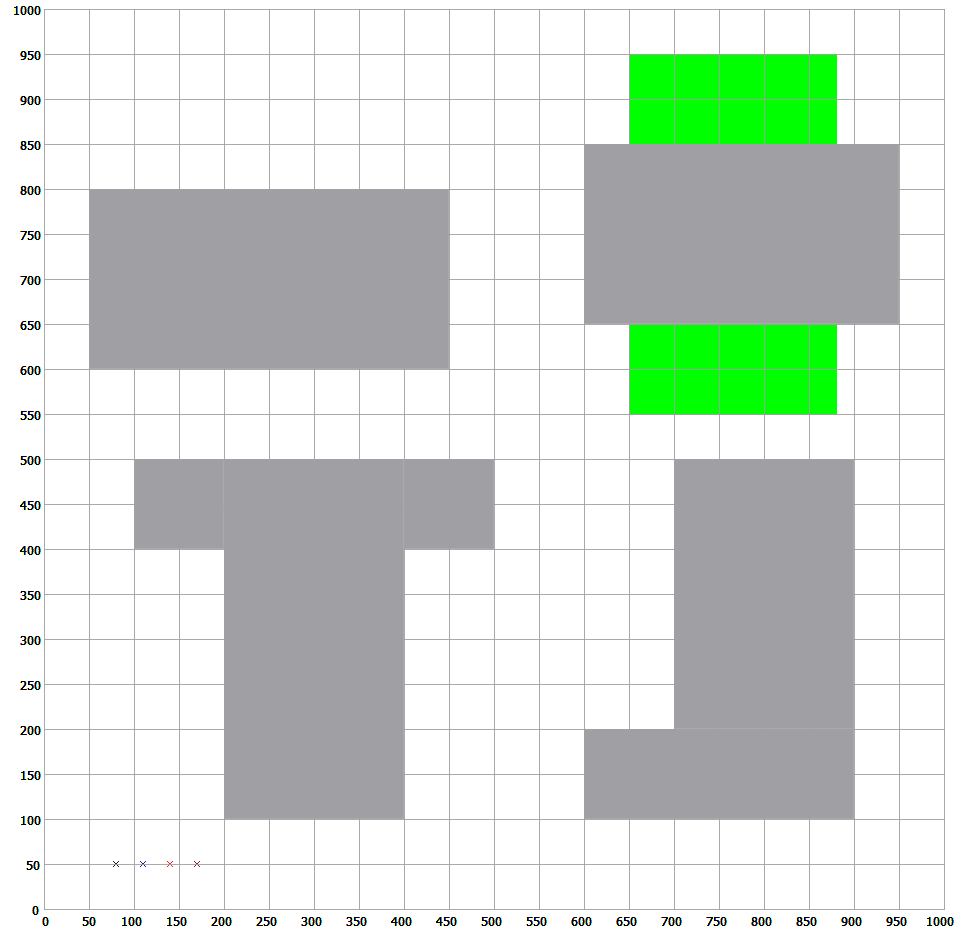
\includegraphics[scale=0.3]{obrazky/map2}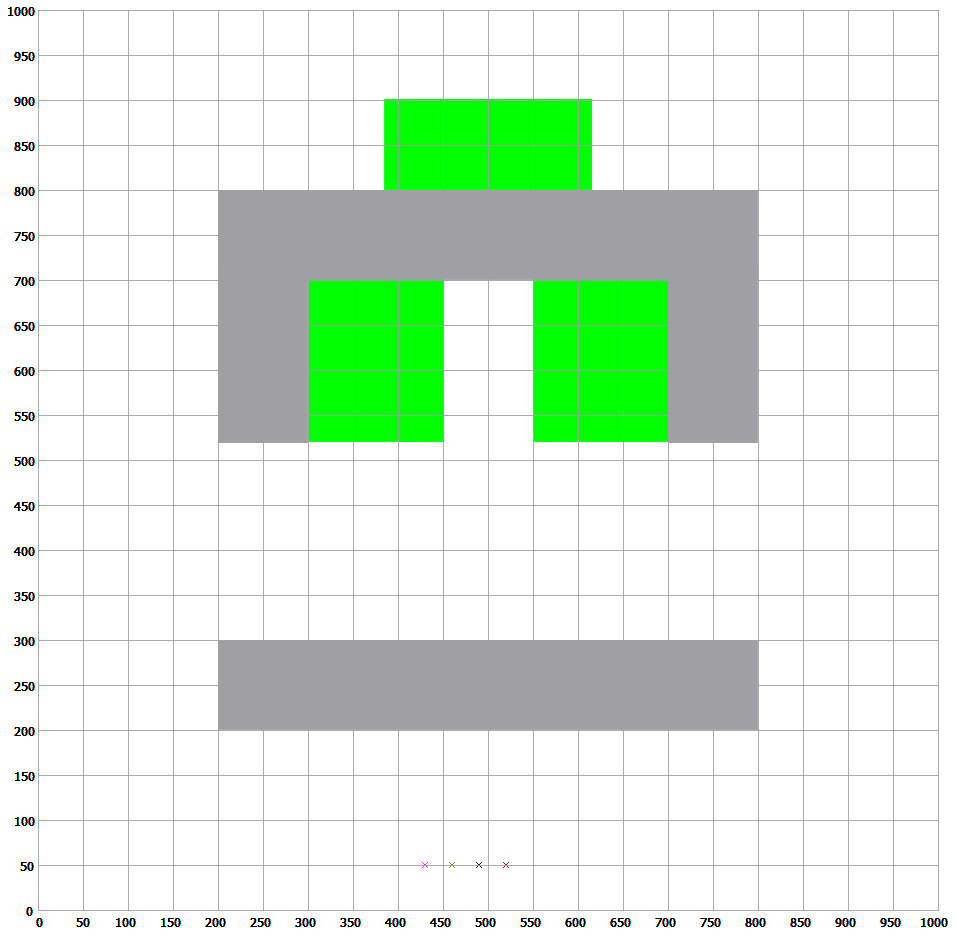
\includegraphics[scale=0.3]{obrazky/map5}

\caption{Maps with goals suitable for grouping \label{fig:Maps-with-goals}}


\end{figure}



\chapter[Paths narrowing]{Paths narrowing\label{chap:Paths-narrowing}}


\chapter[Implementation]{Implementation}

This part will cover implementation of algorithm, which was used for
simulations. Whole codebase can be found at \href{https://github.com/racinmat/AutonomousSurveillanceBachelorThesis}{this github repository}.


\section{External libraries}

In implementation are used some external libries. Every used library
is mentioned here.\href{http://www.boost.org/}{Boost libraries} is
used for smart pointers, libraries for Dubins maneuvers are from Master
Thesis by Petr Váňa\cite{Dubins-thesis}. Generating of JSON from
C++ object is done via \href{http://www.codeproject.com/Articles/20027/JSON-Spirit-A-C-JSON-Parser-Generator-Implemented}{Json Spirit}
library. Another external library is \href{http://gamma.cs.unc.edu/V-COLLIDE/}{V-Collide}
from The University of North Carolina at Chapel Hill. 

Because V-Collide sources were written in 1997 and because I used
C++11 compiler to compile my source codes, I had to rewrite part of
this library for compatibility and to make public API easier to use.
Modifications can be seen in \href{https://github.com/racinmat/VCollide2}{this github repository}. 

Last use external library is QT, which was used to create platform
independent GUI.


\section{Code structure }

Here is shown brief UML scheme demonstrating dependency diagram of
codebase. To keep diagram simple, only services are displayed, other
classes were left out. Diagram was generated using software \href{http://staruml.io/}{StarUML}

\begin{figure}


\caption{Dependency diagram \label{fig:Dependency-diagram}}


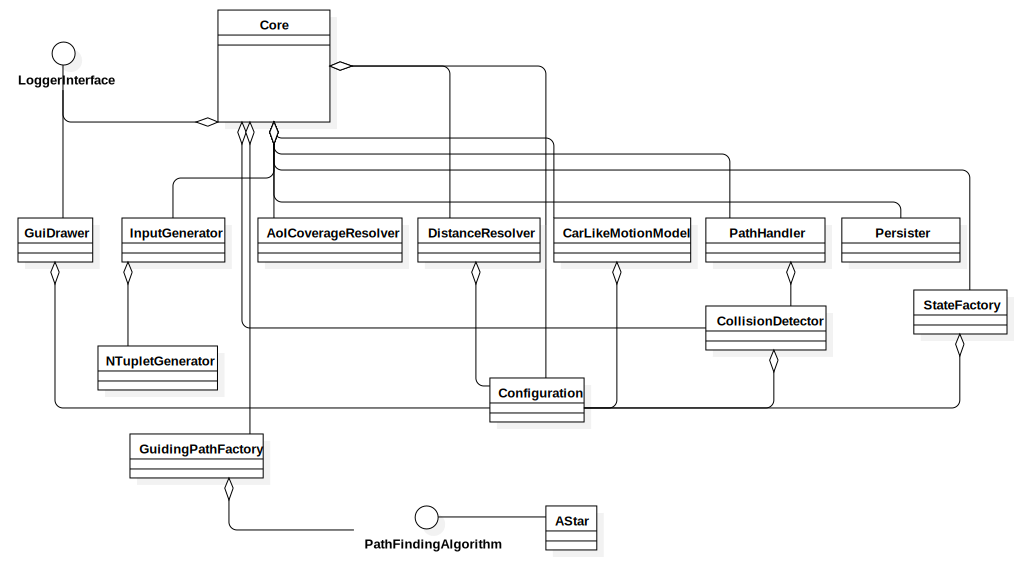
\includegraphics[scale=0.4]{obrazky/umlSchema}
\end{figure}


Core class holds core of whole Application and has all other classes
as dependencies, as is shown in image \ref{fig:Dependency-diagram}. 

State factory creates State classes according to Factory pattern.
State class represents state in RRT-Path algorithm. State has coordinates
and rotations for all UAVs.

Persister persists found path to JSON using Json Spirit library.

PathHandler serves as utils class for manipulations with path (vector
of State classes).

CarLikeMotionModel holds motion model algorithm.
\begin{thebibliography}{1}
\bibitem[1]{Dubins-thesis}Petr Váňa,\emph{ Path Planning for Non-holonomic
Vehicle in Surveillance Missions} {[}online{]}. {[}cit. 2015-12-29{]}.
Dostupný z WWW: \url{https://dspace.cvut.cz/bitstream/handle/10467/61814/F3-DP-2015-Vana-Petr-thesis.pdf}

\end{thebibliography}
\cleardoublepage{}
\end{document}
